\chapter{Psalm 81}

\begin{figure}
  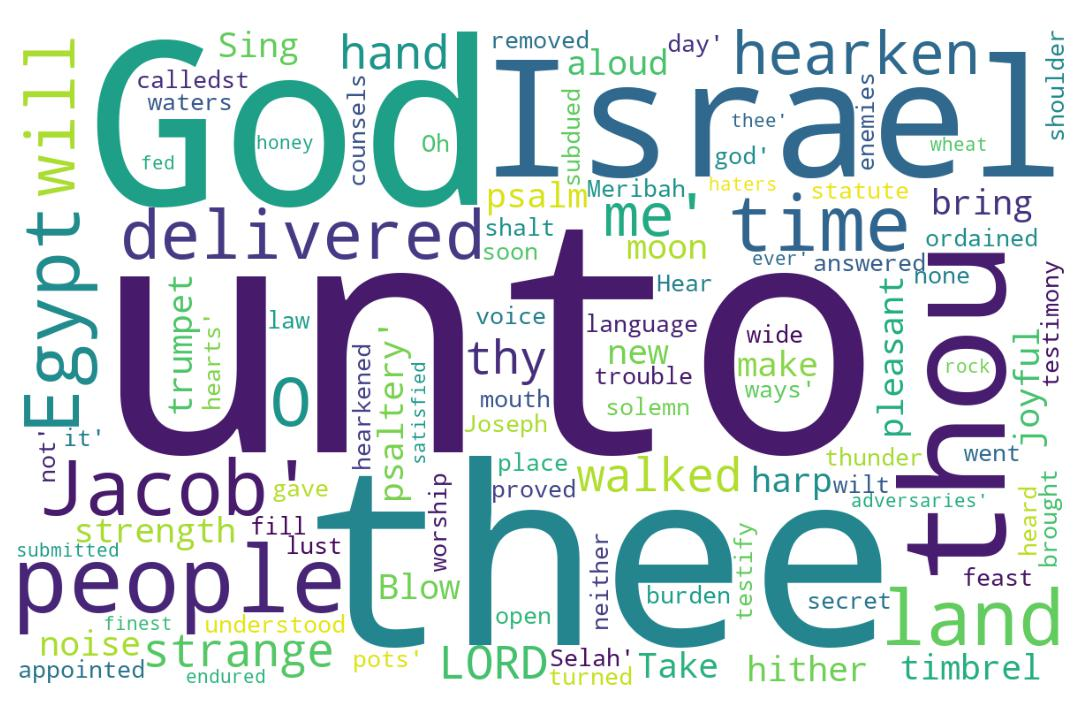
\includegraphics[width=\linewidth]{19OT-Psalms/Psalm81-WordCloud.jpg}
  \caption{Psalm 81 Word Cloud}
  \label{fig:Psalm 81 word Cloud}
\end{figure}



\marginpar{\scriptsize \centering \fcolorbox{bone}{lime}{\textbf{RECOGNIZING ONE'S PLACE}}\\ (Psalm 81) \begin{compactenum}[I.][8]
    \item A \textbf{Call to Rejoice} \index[scripture]{Psalms!Psa 081:01-05}(Psa 81:1-5)
    \item A \textbf{Call to Remember} \index[scripture]{Psalms!Psa 081:06-10}(Psa 81:6-10)
    \item A \textbf{Chains Removed} \index[scripture]{Psalms!Psa 081:06}(Psa 81:6)
    \item The \textbf{Call to be Rescued} \index[scripture]{Psalms!Psa 081:07}(Psa 81:7)
    \item A \textbf{Challenge to Regard God} \index[scripture]{Psalms!Psa 081:08}(Psa 81:8)
    \item A \textbf{Call to Repent} \index[scripture]{Psalms!Psa 081:11-16}(Psa 81:11-16)
\end{compactenum}}




\footnote{\textcolor[rgb]{0.00,0.25,0.00}{\hyperlink{PsalmsTOC}{Return to end of Table of Contents.}}}\footnote{\href{https://audiobible.com/bible/psalms_81.html}{\textcolor[cmyk]{0.99998,1,0,0}{Psalm 81 Audio}}}\textcolor[cmyk]{0.99998,1,0,0}{To the chief Musician upon Gittith, \emph{A Psalm} of Asaph.}\\
\\
\textcolor[cmyk]{0.99998,1,0,0}{Sing aloud unto God our strength: make a joyful noise unto the God of Jacob.} %\footnote{[RUCKMAN]  The first seven verses deal with Israel praising God in its feasts for deliverance from Egypt. The speaker switches from the third person to the first person in the most distracting fashion (vs. 5), where God Himself becomes the speaker in verses 6 and 7. The Psalmist speaks for Israel as “I” in verse 5 (“I heard a language that I understood not”), but immediately places Israel into the second person (“Thou calledst in trouble”), and then speaks for God as “I” (“I delivered thee; I answered thee”). The only other way out is to claim that the “I” of “I heard a language that I understood not” matches Hosea 8:4 and Amos 3:2. It is possible for God to speak of not knowing something that happens right in front of His face. Observe: “I never knew you: depart from me” (Matt. 7:23). Obviously God knows every man’s birth, life, death, thoughts, background, feelings, words, ideas, imaginations, motives, works, and beliefs; but still: “I never knew you.” Thus “I heard a language that I understood not” (vs. 5). However, the former meaning is probably correct; very often a prophet will switch persons. \cite{Ruckman1992Psalms}  }
[2] \textcolor[cmyk]{0.99998,1,0,0}{Take a psalm, and bring hither the timbrel, the pleasant harp with the psaltery.}
[3] \textcolor[cmyk]{0.99998,1,0,0}{Blow up the trumpet in the new moon, in the time appointed, on our solemn feast day.} %\footnote{[RUCKMAN] The “solemn feast day” (vs. 3) is the date of the Second Advent. This date is the Feast of Tabernacles (see 2 Chron. 7:9; Neh. 8:18; Hosea 9:5, 12:9; Lev. 23:34; Deut. 16:13; 31:10; 2 Chron. 8:13; and Ezra 3:4). This is THE outstanding date on the calendar of history from 4000 B.C. to A.D. 2000, for it dates BOTH ADVENTS and is commemorated once a year by the sun itself, which is four days off center from the earth’s orbit; these days are September 20, 21, 22, and 23. The “statute” and “law” that was “ordained” (vss. 4--5) was to confirm the appearance of Jesus Christ after the Marriage of the Lamb (see comments under Ps. 19:4--5). All the commentators....etc., etc. \cite{Ruckman1992Psalms} }
[4] \textcolor[cmyk]{0.99998,1,0,0}{For this \emph{was} a statute for Israel, \emph{and} a law of the God of Jacob.}
[5] \textcolor[cmyk]{0.99998,1,0,0}{This he ordained in Joseph \emph{for} a testimony, when he went out through the land of Egypt: \emph{where} I heard a language \emph{that} I understood not.}
[6] \textcolor[cmyk]{0.99998,1,0,0}{I removed his shoulder from the burden: his hands were delivered from the pots.}
[7] \textcolor[cmyk]{0.99998,1,0,0}{Thou calledst in trouble, and I delivered thee; I answered thee in the secret place of thunder: I proved thee at the waters of Meribah. Selah.} %\footnote{[RUCKMAN]  Verse 7 was an answer to Psalm 50:15. “The secret place of thunder” would be Mt. Sinai (see Exodus 19:16 and 20:18), although the thing will be repeated in the Tribulation (1 Samuel 2:10). You say, “Where do you get THAT from?” That’s easy—“Selah” (vs. 7), right in front of the noses of the Scholar’s Union. You know what they did with it, and you don’t have to be told. Revelation 10:3 and 16:18 are not in the Book to be ignored. The rebuke that God gives Israel, here, was prefaced by verse 7, which said, “I proved thee at the waters of Meribah.” This was Israel’s sin (see Exod. 17:3–7), and it is described in much detail in our Bible Believer’s Commentary on Exodus. “Hear, O my people” (vs. 8), as in 78:1. Nothing that follows is difficult. It was discussed in The Bible Believer’s Commentary on Exodus, which see. \cite{Ruckman1992Psalms} }
[8] \textcolor[cmyk]{0.99998,1,0,0}{Hear, O my people, and I will testify unto thee: O Israel, if thou wilt hearken unto me;}
[9] \textcolor[cmyk]{0.99998,1,0,0}{There shall no strange god be in thee; neither shalt thou worship any strange god.}
[10] \textcolor[cmyk]{0.99998,1,0,0}{I \emph{am} the LORD thy God, which brought thee out of the land of Egypt: open thy mouth wide, and I will fill it.} %\footnote{God will fill their mouths (vs. 10) as a mother eagle will fill the mouth of an offspring, for He brought them out ``on eagles’ wings'' (Exod. 19:4).}
[11] \textcolor[cmyk]{0.99998,1,0,0}{But my people would not hearken to my voice; and Israel would none of me.}
[12] \textcolor[cmyk]{0.99998,1,0,0}{So I gave them up unto their own hearts' lust: \emph{and} they walked in their own counsels.}
[13] \textcolor[cmyk]{0.99998,1,0,0}{Oh that my people had hearkened unto me, \emph{and} Israel had walked in my ways!}
[14] \textcolor[cmyk]{0.99998,1,0,0}{I should soon have subdued their enemies, and turned my hand against their adversaries.}
[15] \textcolor[cmyk]{0.99998,1,0,0}{The haters of the LORD should have submitted themselves unto him: but their time should have endured for ever.}
[16] \textcolor[cmyk]{0.99998,1,0,0}{He should have fed them also with the finest of the wheat: and with honey out of the rock should I have satisfied thee.} %\footnote{Observe the apparent contradiction between verse 16 and Deuteronomy 32:13. One verse said that God did feed them with those items, and the other said He would have if they had obeyed Him. Jamieson, Fausset, Brown, and Kroll find the reference in Deuteronomy, but not knowing what on earth either passage is about, they pretend that there isn’t any problem. Now God testifies against His people. His complaint is the same complaint voiced by Joshua when Israel entered the Promised Land (Josh. 24:14, 19). It is the same complaint and warning that God gave them before they left the wilderness. Turning a deaf ear to this warning is the thing that caused both Israel (2 Kings 18) and Judah (Jer. 39–- 40) to go into captivity: “there shall no strange god be in thee” (vs. 9). God “gave them up” (vs. 12) like He gave up the Gentiles in Romans 1:24–25. Stephen describes this very thing in Acts 7:42. The “they” and “their” in the passage (vss. 12, 14) is Israel, but the “them” of verse 16 is in contrast with the “thee” of verse 16.  This produces a strange thing among the commentators. “Their time” is given to God’s enemies in the NIV and the RSV, but the same expression is attributed to Israel by Jamieson, Fausset, Brown, and Spurgeon. (Kroll wisely keeps his mouth shut so no one will spot his ignorance: Prov. 17:28). The ASV leaves the text as it stands in the AV, but the NKJV (Curtis Hutson, Harold Okenga, James Price, F. F. Bruce, et al.) goes along with the RSV of the National Council of Churches and writes “their fate,” without identifying WHOSE fate. The Living Bible says it is the enemy’s fate, and so do the RSV, NRSV, and NIV. But they could have changed  it. They would have “submitted themselves unto” the Lord. If they had done this, then they would have fed on what Israel fed on in Deuteronomy 32:13. The enemies would not have just been “subdued” (vs. 14), they would have “submitted” themselves to God and Israel, so they would have shared in Israel’s physical and material blessings. Note the Holy Spirit’s comments on this in Romans 11:12, which all the...you know by now! “He should have fed them”—the enemies that God subdued and came into submission —with the things that He fed Israel (see vs. 10). “He should have fed them also” clinches the case. Of course, we can find all kinds of spiritual truths in the Psalm.
%\begin{compactenum}
%\item We got saved when we were “in trouble,” and at that time we called upon the name of the Lord (vs. 7). 
%\item Testings followed our salvation (vs. 7).
%\item From that point on, we were to listen to God, not to man (vs. 8), and since “covetousness...is idolatry” (Col. 3:5), we were to have no “strange gods” (vs. 9).
%\item God will provide FOOD (vs. 10 with 1 Tim. 6:8).
%\item God will fight for us if we yield to Him (vss. 13--14).
%\item Conversions will follow our obedience (vs. 15).
%\item And the converted enemies of God (see Rom. 5:10) would enjoy “honey out of the rock” (see 1 Pet. 2:3).
%\end{compactenum} }

